\section{Assessment of social force models}
% TODO: Add a discussion about the "toy model" thing. Go through the whole 
% section looking at structure, coherency etc.
% Come up with a concept for the section and make it so.
\label{sec:assessment}
When we started to implement and simulate the model we found some fault
in the model, which gave rise to some ideas of how we make the model better.
These minor fault in the model and the solutions to have we could improve it
is described in this section.

\subsection{The repulsive force between agents in three-dimensional space}
From the given formula for calculating the repulsive force between agents in the 
description of the model, the part calculating the force to keep the personal space 
can be omitted when the agents are rather close to each other, then the calculation 
can be reduced as Equation (\ref{eq:re}).

\begin{equation}\label{eq:re}
\overrightarrow{f_{\alpha\beta}}(t) = A_{\alpha}^{2} exp\left[ \frac{r_{\alpha\beta} - d_{\alpha}\beta}{B_{\alpha}^{2}}\right]  \overrightarrow{n_{\alpha\beta}}
\end{equation}

Taking the norms of both sides of Equation (\ref{eq:re}), we can draw the relation 
between the value of $\overrightarrow{f_{\alpha\beta}}(t)$ and $d_{\alpha \beta}$, 
as in Figure (\ref{fig:physicalinteraction})
\\
\begin{figure}
\centering
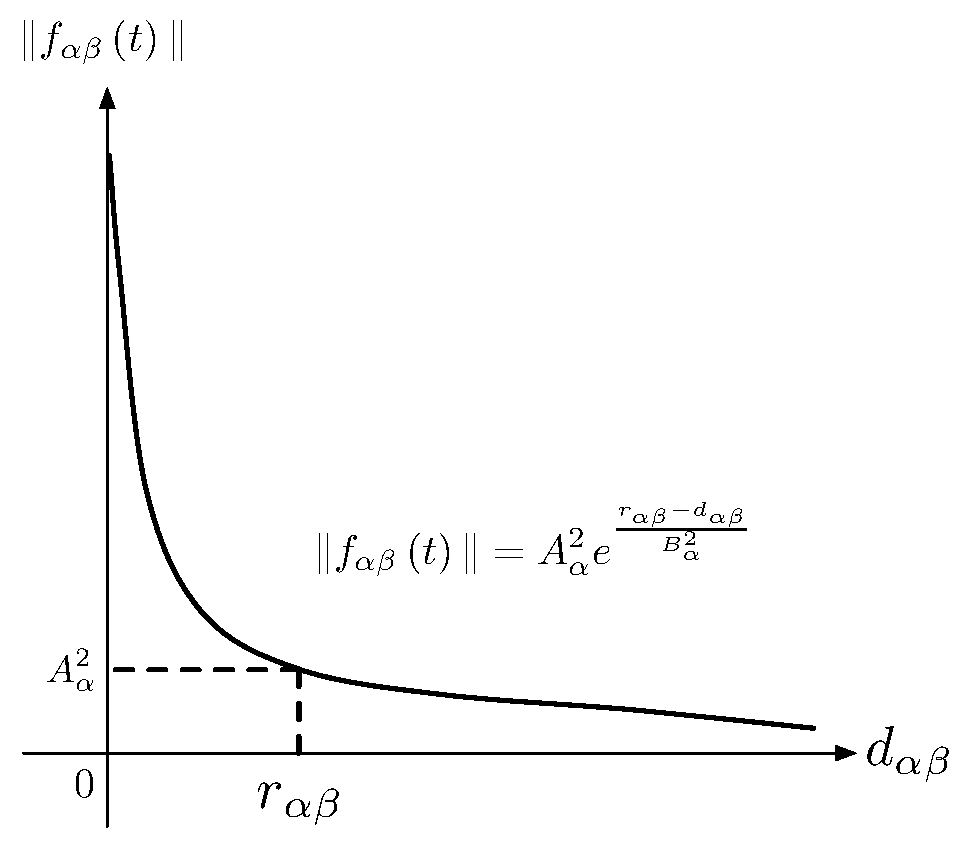
\includegraphics[scale=0.45]{Figures/physicalinteraction.pdf} 
\caption{The function about the interaction force $\vec{f_{\alpha\beta}}(t)$ and the distance between two agents
$d_{\alpha\beta}$ }\label{fig:physicalinteraction}
\end{figure}

There is one intersection of the graph and the axis $ \left( 0, A_{\alpha}^{2} exp\left( \frac{r_{\alpha\beta} }{B_{\alpha}^{2}}\right)  \right) $. 
If put into the constants, we will be able to get a maximum value of $ f_{\alpha\beta}(t) $, 
since the distance between agents cannot be negative. Here we set $ A_{\alpha}^{2} = 3 m/s^{2} $, 
$ r_{\alpha\beta} = 0.6 m $, and $ B_{\alpha}^{2} = 0.2 m $, so $ f_{\alpha\beta}(t)^{max} \doteq 60 m/s^{2} $, 
which is about six times the gravitational acceleration and represents a rather 
large force between agents (as large as six person's weight).

However, we notice that the effective part of the force calculated above is only the horizontal 
component that enables the agent to move horizontally in the plane where we do the simulation, 
but the reality is that the agents sometimes are also able to move vertically, for example, 
by stepping upon other people when they cannot take the pushing force from the surrounding agents. 
When that happens, the horizontal component of the repulsive force becomes smaller even if 
$d_{\alpha\beta}$ is kept the same.	
Therefore, a qualitative modification of dependence between $ f_{\alpha\beta}(t) $ 
and $ d_{\alpha\beta} $ could be:

\begin{figure}[hb]   
\centering
    {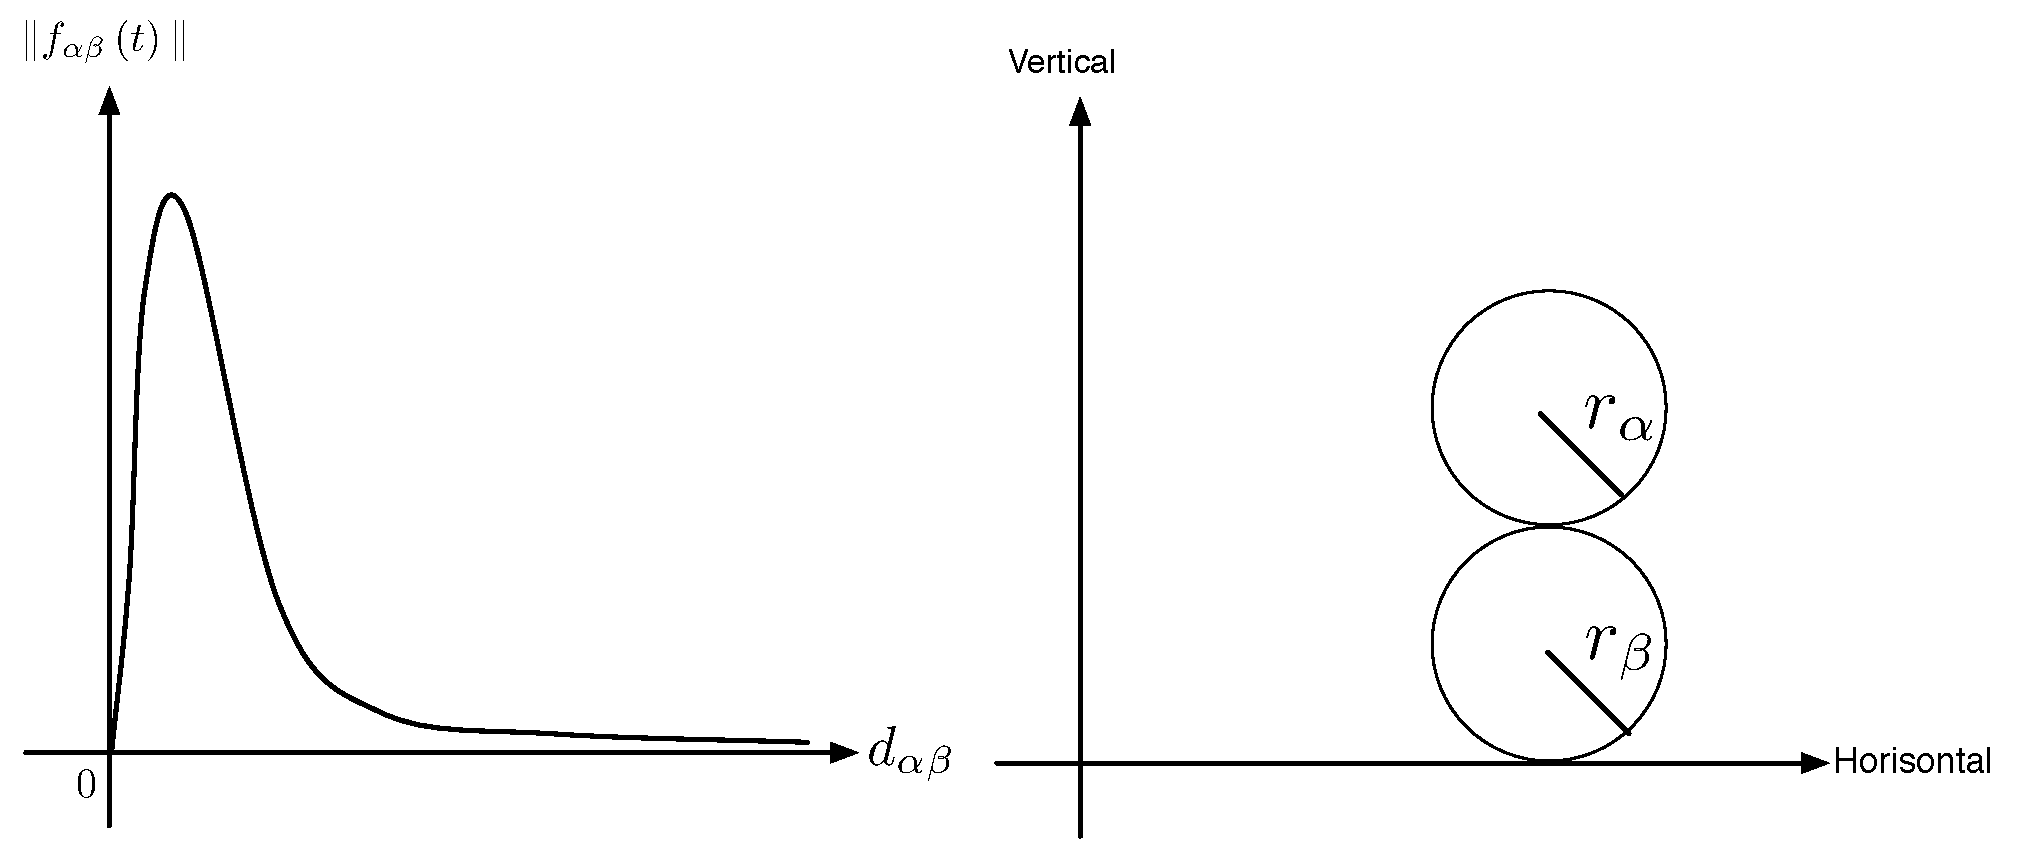
\includegraphics[scale=0.35]{Figures/ForceOverlapping.pdf}} 
    \caption{}
    \label{forceoverlapping}
\end{figure}
 

\subsection{Limitations of social force models}
In this section we discuss the different features of the model, problems when 
computing the model, limits of the model and ways of improving the model that 
we thought of when we went into more details of the model and started to 
simulate it.

There are several limitations the model that we encountered when we started 
analyse and simulate the model. In this section we discuss some relevant 
limitations of the model that we thought of.

The flexibility of the model in the sence that which situations it could model 
and some limitations of the agents and their awareness of the environment.
E. g. (Comparison article) some people fall in panic situations and become 
obstacles for other people, which is not a feature this model deals with. In 
our model none of the agents fall and become an obstacle force other agents as 
would be seen in real life panic situations.

Another flaw in the model is that the agents do not have way finding, which 
mean that they can not escape a more complex environment with a lot of rooms 
and corridors. As it is now we can only simulate simple cases as the squared 
room and the corridor.  An improvement of the model would then be to implement 
way finding for the agents, so that they can manoeuvre around in other more 
complex cases then the ones we have.

In other models as the HiDAC, agents can share information about the 
environment, such that the agents have a better idea of where the exit is/are 
(Comparison article). In a real panic situation you would expect people to 
communicate when evacuation a building.

Other models take into account herding behavior between the agents  
\cite{helbing00}, so that some people have tendency to follow other agents, 
while other agents have a tendency to go their own way,  and by doing so 
explore the environment for possible exits.

As the model is now there is no friction between the agents, so that agents 
that have higher velocity than the ones standing in their path, can slide in 
between slower moving agents in front of them, without them slowing down when 
they slide by. In real case scenario people would not slip by that easily 
since the friction between the people would slow them down.  Without friction 
between agents there would be less clogging in front of doors, and the time it 
takes the agents to exit a room would be less than the time expected. Thus the 
validation of the would not be as good as if there would be friction between 
the agents.

At the moment we can not simulate a case where the visibility is very low. The 
agents have a way point to follow, but if the visibility only is 1 meter, e. 
g. in a smoke filled room, the  agents would not have way point to follow, and 
hence round around with out purpose. Here the tangential forces would also 
help the agent to find the exit, but navigation through the tangential force 
from the walls.

\subsection{social force in crowd modelling}
%-take a step back, discuss the model in general terms
%-is social force a good way to discuss this 
%-incomplete description, inherent in types of paper
At this point we have got some understanding of the social force model, and 
also given our opinion about the limitation of the model. We cannot help to 
think about the same question as we point out in the introduction, whether 
social force is a proper measure of crowd behaviour. 

While searching for articles leading to social force model, we see there is a 
evolutionary path in transferring physical concepts to describe crowd dynamics.
The success of using fluid dynamics thoughts to model traffic problem encourages 
people to bring the same measurement to model crowd. 
Later, Helbing improves that way by combining the fluid dynamic and gas kinetics 
concepts. \cite{social-force} However, in order to add the self-organized feature 
into account, it is necessary to use the agent-based concept.  At the same time, 
use certain quantity to measure the desire of each agent, and the social force model 
transfer the "social force" into the calculation in the actual acceleration, which may
arise problems because many laws in physics does not apply in this model. 
There is a common feature of the social force model articles, that the method for 
justifying the model is mostly by comparing with observations. It is not 
similar with many cases in classical mechanics, when talking of forces people 
always evaluate energy and momentum, but it is not possible when we have 
the social force involved.
